\chapter{Исследовательский раздел}
В данном разделе проведено исследование точности разработанной модели рекомендаций в зависимости от её устройства.
Таким образом, получена возможность правильно выбрать модель машинного обучения.

\section{Проведение измерений точности}
Для получения точности исследуемых моделей проведены следующие шаги:
\begin{itemize}
	\item реализована модель, соответствующая заданному набору параметров;
	\item реализовано чтение тестовых данных, где количество оценок пользователя хотя бы $10$;
	\item проведены предсказания оценок на тестовых данных;
	\item вычислены модули разности между полученными оценками и эталонными, получился массив ошибок;
	\item вычислен процент ошибок, меньших $0{.}5$;
	\item вычислен процент ошибок $p_1$ лежащих, в промежутке $[0{.}5; 1)$;
	\item вычислен процент ошибок $p_2$ не меньших $1$;
	\item точность вычислена как $p_1 + p_2$.
\end{itemize}
Принято, что если разность между предсказанной оценкой рецепта и той оценкой, которую реально выставил пользователь, менее $1$, то система не порекомендует то, что пользователю не нравится, так как при округлении предсказанной оценки ошибка составит не более $1$.
Поэтому модели сравниваются по проценту тестовых случаев, когда предсказанная оценка отличается от реальной на менее, чем $1$.
Опытным путём установлено, что при случайном угадывании оценок точное предсказание случается в $17\%$, а ошибка на $1$ -- в $16\%$.
Это позволит более наглядно показать, что реализованные модели действительно предсказывают оценку, а не угадывают её.

\subsection{Регрессионная модель}
\subsubsection{Подбор параметров модели}
Рассматривается алгоритм рекомендаций, описанный в конструкторском разделе работы.
Для проведения измерений необходимо сформулировать, какие именно характеристики модели будут меняться.
К выделенным параметрам относится:
\begin{itemize}
	\item метрика близости векторов;
	\item вид регрессии;
	\item параметры регуляризации.
\end{itemize}
В таблице~\ref{tab:reg_model} представлены результаты тестирования регрессионной модели с различными параметрами на точность.
В первом столбце данной таблицы -- количество оценок в выборке для обучения модели, во втором -- регуляризационный параметр.
Следующие $2$ столбца отображают процент тестовых случаев с какой-либо ошибкой.
В последнем столбце представлены результаты вычисления сформулированной метрики качества -- точности.

\begin{table}[H]
\centering
\begin{tabular}{|l|c|c|c|c|}
\hline
\thead{\small Оценки} & \thead{\small Рег. \\ парам.} & \thead{\small Ошибка \\ $< 0{.}5$} & \thead{\small Ошибка\\$[0{.}5;1)$} & \thead{\small Точность} \\
\hline
$\geqslant 10$ & 0 & $44{.}08$ & $20{.}48$ & $64{.}88$ \\ \hline
$\geqslant 10$ & $0{.}5$ & $52{.}66$ & $27{.}64$ & $80{.}3$ \\ \hline
$\geqslant 10$ & $1{.}0$ & $54{.}23$ & $28{.}49$ & $82{.}72$ \\ \hline
$\geqslant 10$ & $2{.}0$ & $55{.}36$ & $28{.}87$ & $84{.}23$ \\ \hline
$\geqslant 10$ & $4{.}0$ & $55{.}77$ & $28{.}93$ & $84{.}7$ \\ \hline
$\geqslant 10$ & $8{.}0$ & $56{.}24$ & $28{.}71$ & $84{.}95$ \\ \hline
$\geqslant 10$ & $10$ & $56{.}26$ & $28{.}69$ & $84{.}95$ \\ \hline
$\geqslant 10$ & $11$ & $56{.}28$ & $28{.}69$ & $84{.}97$ \\ \hline
$\geqslant 10$ & $12$ & $56{.}26$ & $28{.}71$ & $84{.}97$ \\ \hline
$\geqslant 10$ & $16$ & $56{.}23$ & $28{.}75$ & $84{.}98$ \\ \hline

$3$ -- $9$ & 0 & $51{.}54$ & $10{.}11$ & $61{.}65$ \\ \hline
$3$ -- $9$ & $0{.}5$ & $51{.}02$ & $17{.}23$ & $68{.}25$ \\ \hline
 $3$ -- $9$ & $1{.}0$ & $51{.}21$ & $18{.}75$ & $69{.}96$ \\ \hline
$3$ -- $9$ & $2{.}0$ & $51{.}27$ & $20{.}07$ & $71{.}34$ \\ \hline
$3$ -- $9$ & $4{.}0$ & $51{.}76$ & $20{.}78$ & $72{.}54$ \\ \hline
$3$ -- $9$ & $8{.}0$ & $51{.}95$ & $20{.}63$ & $72{.}58$ \\ \hline
$3$ -- $9$ & $10$ & $51{.}97$ & $20{.}59$ & $72{.}56$ \\ \hline
$3$ -- $9$ & $11$ & $51{.}99$ & $20{.}57$ & $72{.}56$ \\ \hline
$3$ -- $9$ & $12$ & $51{.}99$ & $20{.}57$ & $72{.}56$ \\ \hline
$3$ -- $9$ & $16$ & $52{.}03$ & $20{.}53$ & $72{.}56$ \\ \hline
\end{tabular}
\caption{\centering Результаты измерения точности регрессионных моделей }
\label{tab:reg_model}
\end{table}
В результате тестирования видно, что наиболее предпочтительный для использования вариант -- модель, использующая Евклидову метрику для определения входных параметров регрессии и линейную регрессию с коэффициентом регуляризации $11$.
Примерно в  $85\%$ случаев она ошибается не более, чем на $1$, что в $2{.}5$ раза лучше случайного угадывания оценки.

\subsection{Метод $k$ ближайших соседей}
Далее рассмотрен алгоритм рекомендаций <<$k$ ближайших соседей>>.
При его тестировании варьировалось значение $k$ и метрика близости векторов.
Также проведено тестирование модели при уменьшении количества размерностей вектора рецепта с помощью вычисления профиля пользователя.
Результаты измерений характеристик разработанного рекомендательного алгоритма представлены в таблице~\ref{tab:knn_model}.
В первом столбце указана используемая метрика расстояния между векторами, во втором -- значение $k$, а в третьем -- применялось ли уменьшение размерностей вектора рецепта.
В следующих $2$ столбцах приведены проценты тестовых случаев с определённой ошибкой.
Результат вычисления точности модели представлен в последнем столбце данной таблицы.

\begin{table}[H]
\centering
\begin{tabular}{|l|c|c|c|c|c|}
\hline
\thead{Метрика} & \thead{k} & \thead{Уменьшение\\размерности} & \thead{Ошибка \\ $< 0{.}5$} & \thead{Ошибка \\ $[0{.}5;1)$} & \thead{Точность}\\
\hline
кос. подобие & $2$ & $-$ & $42{.}44$ & $21{.}86$ & $64{.}3$ \\ \hline
кос. подобие & $3$ & $-$ & $54{.}47$ & $14{.}06$ & $68{.}53$ \\ \hline
кос. подобие & $4$ & $-$ & $46{.}46$ & $25{.}03$ & $71{.}49$ \\ \hline
кос. подобие & $5$ & $-$ & $52{.}37$ & $19{.}69$ & $72{.}06$ \\ \hline
кос. подобие & $6$ & $-$ & $47{.}6$ & $27{.}73$ & $75{.}33$ \\ \hline
кос. подобие & $7$ & $-$ & $53{.}09$ & $25{.}65$ & $78{.}74$ \\ \hline
кос. подобие & $8$ & $-$ & $48{.}29$ & $31{.}56$ & $79{.}85$ \\ \hline
кос. подобие & $9$ & $-$ & $52{.}99$ & $27{.}47$ & $80{.}46$ \\ \hline
кос. подобие & $10$ & $-$ & $49{.}09$ & $31{.}83$ & $80{.}92$ \\ \hline

Евклидова & $2$ & $-$ & $43{.}82$ & $22{.}03$ & $65{.}85$ \\ \hline
Евклидова & $3$ & $-$ & $54{.}57$ & $15{.}18$ & $69{.}75$ \\ \hline
Евклидова & $4$ & $-$ & $46{.}94$ & $24{.}45$ & $71{.}39$ \\ \hline
Евклидова & $5$ & $-$ & $54{.}0$ & $19{.}51$ & $73{.}51$ \\ \hline
Евклидова & $6$ & $-$ & $48{.}96$ & $28{.}01$ & $76{.}97$ \\ \hline
Евклидова & $7$ & $-$ & $53{.}93$ & $25{.}12$ & $79{.}05$ \\ \hline
Евклидова & $8$ & $-$ & $49{.}56$ & $30{.}39$ & $79{.}95$ \\ \hline
Евклидова & $9$ & $-$ & $53{.}09$ & $27{.}97$ & $81{.}06$ \\ \hline
Евклидова & $10$ & $-$ & $49{.}73$ & $31{.}87$ & $81{.}6$ \\ \hline

кос. подобие & $5$ & $+$ & $61{.}32$ & $26{.}57$ & $87{.}89$ \\ \hline
кос. подобие & $6$ & $+$ & $61{.}46$ & $26{.}48$ & $87{.}94$ \\ \hline
кос. подобие & $7$ & $+$ & $62{.}37$ & $26{.}54$ & $88{.}91$ \\ \hline
кос. подобие & $8$ & $+$ & $62{.}52$ & $26{.}39$ & $88{.}91$ \\ \hline
кос. подобие & $9$ & $+$ & $63{.}2$ & $26{.}05$ & $89{.}25$ \\ \hline
кос. подобие & $10$ & $+$ & $63{.}15$ & $26{.}17$ & $89{.}32$ \\ \hline

Евклидова & $5$ & $+$ & $61{.}63$ & $24{.}07$ & $85{.}7$ \\ \hline
Евклидова & $6$ & $+$ & $61{.}43$ & $24{.}31$ & $85{.}74$ \\ \hline
Евклидова & $7$ & $+$ & $62{.}84$ & $24{.}67$ & $87{.}51$ \\ \hline
Евклидова & $8$ & $+$ & $62{.}91$ & $24{.}58$ & $87{.}49$ \\ \hline
Евклидова & $9$ & $+$ & $63{.}37$ & $25{.}0$ & $88{.}37$ \\ \hline
Евклидова & $10$ & $+$ & $63{.}4$ & $25{.}09$ & $88{.}49$ \\ \hline
\end{tabular}
\caption{\centering Результаты измерения точности модели <<$k$ ближайших соседей>> }
\label{tab:knn_model}
\end{table}

В результате тестирования модели <<$k$ ближайших соседей>> установлено, что чем больше значение $k$, тем больше предсказанных оценок отличаются от эталонных не более, чем на $1$.
Относительно сформулированной метрики наиболее предпочтительно использовать $k \geqslant 10$, Евклидово расстояние и уменьшение размерности вектора рецепта с помощью вычисления профиля пользователя.
Однако значение $k$ не может постоянно расти, так как количество оценок пользователя должно быть не менее $k$.
Более того, чем больше $k$, тем больше времени потребуется на рекомендацию из-за асимптотики алгоритма.
Таким образом, алгоритм <<$k$ ближайших соседей>> применим в том случае, когда количество оценок пользователя хотя бы $10$ и $k \geqslant 10$.
Постоянно увеличивать $k$ не представляется возможным, и максимальное его значение зависит от временных ограничений. 

\section{Графики метрик моделей}
\subsection{Вычисление метрик}
Далее на рисунках~\ref{fig:reg_metric}--\ref{fig:knn_metric_2} представлены следующие метрики качества моделей:
\begin{itemize}
	\item <<MSE>>, формула~\eqref{eq:mse};
	\item <<MAE>>, формула~\eqref{eq:mae};
	\item медианная ошибка;
	\item максимальная ошибка;
	\item средняя ошибка;
	\item часть оценок, предсказанных с точностью до $1$.
\end{itemize}

\begin{figure}[H]
	\centering
	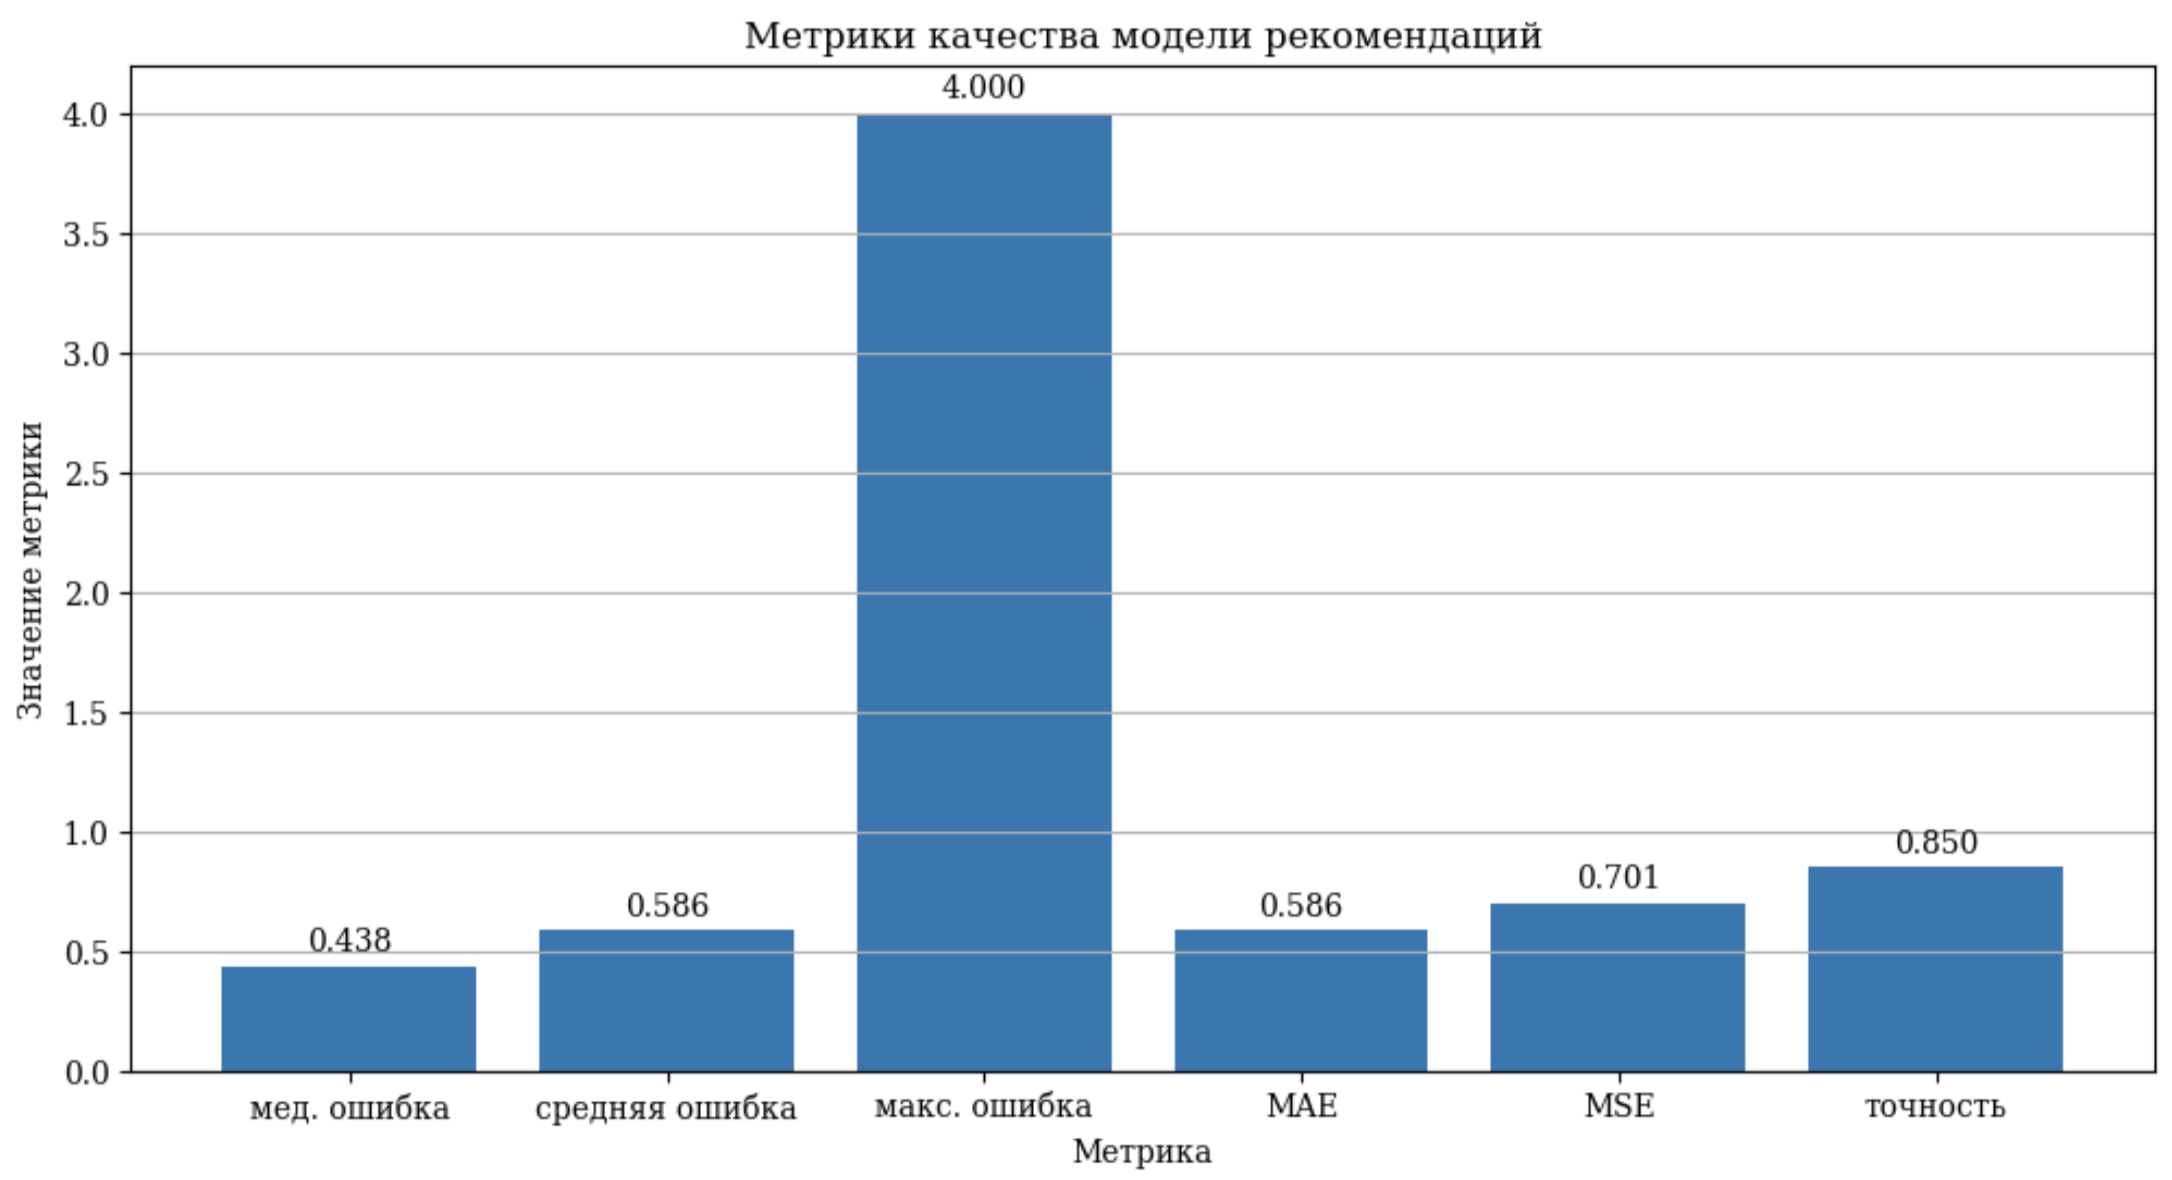
\includegraphics[width=\textwidth]{img/reg_metric.png}
	\caption{
	    Результат вычисления метрик качества регрессионной модели при коэффициенте регуляризации $\alpha=11$
	}
	\label{fig:reg_metric}
\end{figure}
\begin{figure}[H]
	\centering
	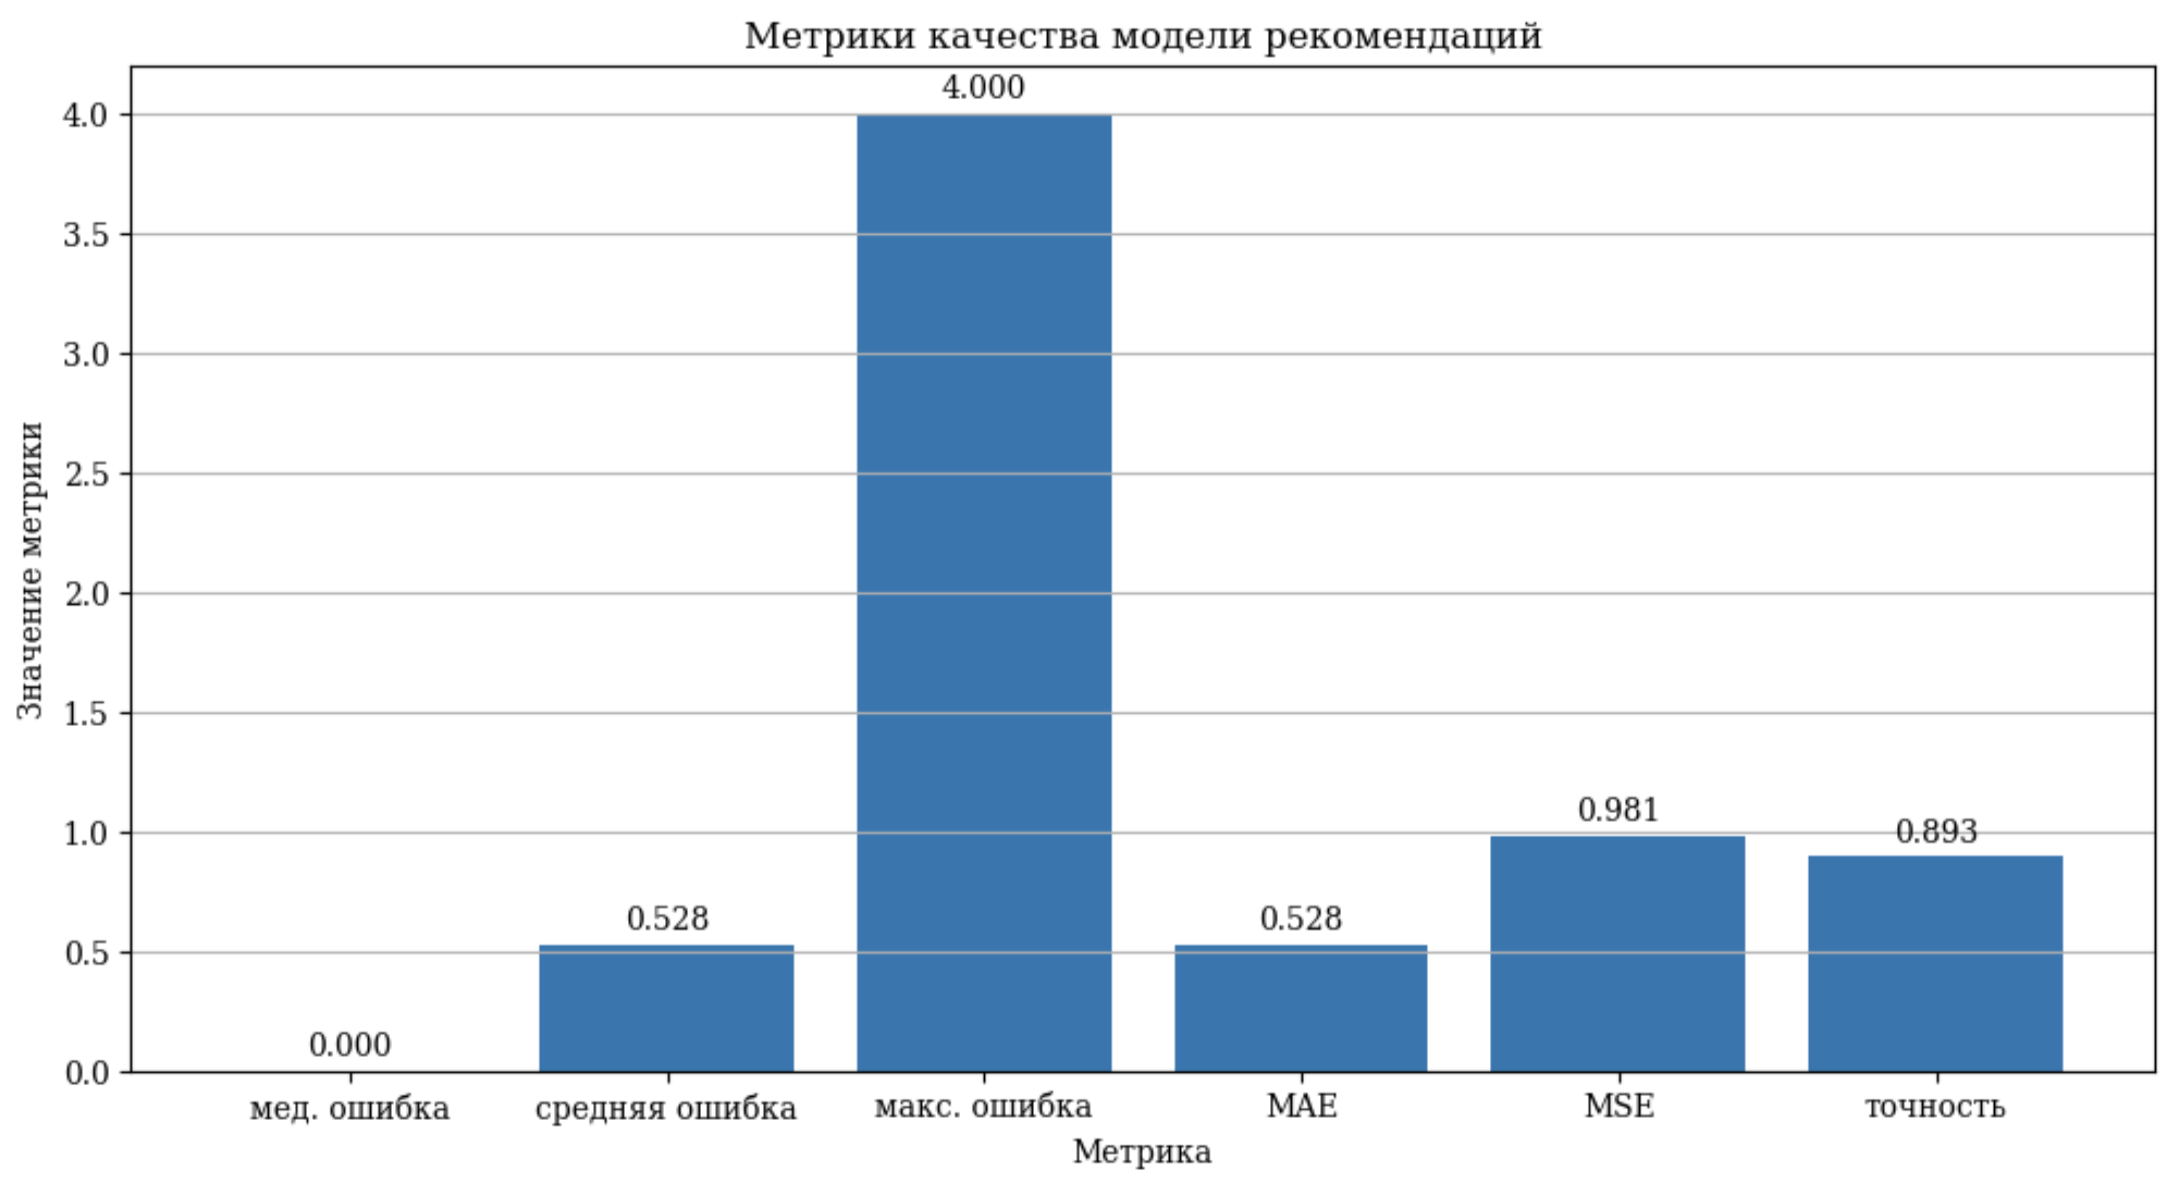
\includegraphics[width=\textwidth]{img/knn_metric_1.png}
	\caption{
	    Результат вычисления метрик качества модели <<$k$ ближайших соседей>> при использовании $k = 10$, Евклидового расстояния и уменьшения размерности вектора с помощью вычисления профиля пользователя
	}
	\label{fig:knn_metric_1}
\end{figure}
\begin{figure}[H]
	\centering
	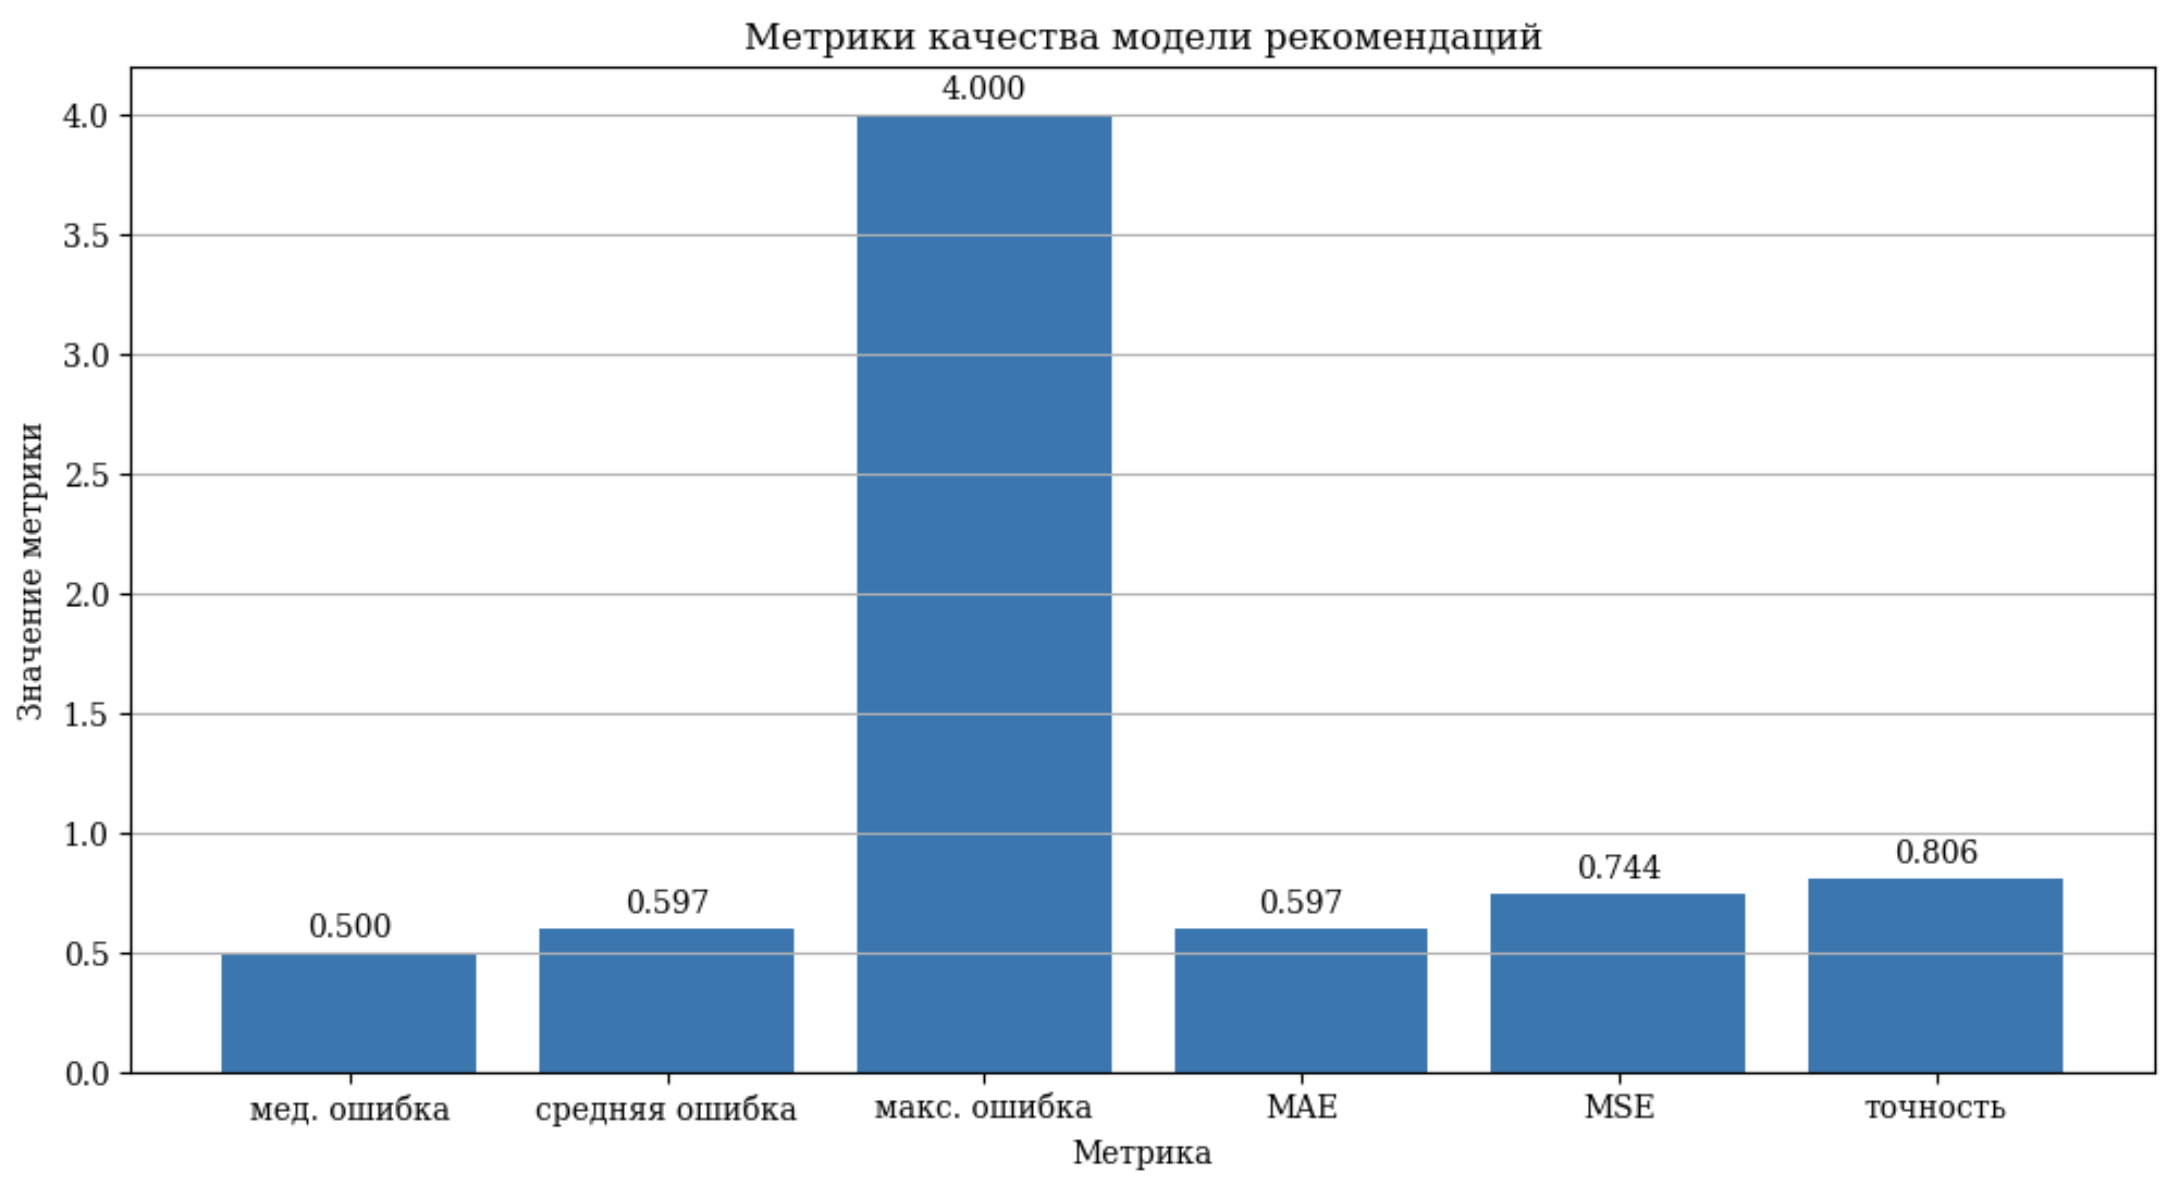
\includegraphics[width=\textwidth]{img/knn_metric_2.png}
	\caption{
	    Результат вычисления метрик качества модели <<$k$ ближайших соседей>> при использовании $k = 10$, Евклидового расстояния и без уменьшения размерности вектора
	}
	\label{fig:knn_metric_2}
\end{figure}
\begin{equation}
    \label{eq:mae}
    \mathrm{MAE} = \frac{\sum\limits_{i=1}^{n} |\hat{y}_i - y_i|}{n},
\end{equation}
где $n$ -- количество тестовых случаев, а  $\hat{y}_i$ и  $y_i$ -- предсказанное и эталонное значения соответственно.

\subsection{Анализ результатов}
В результате вычисления метрик установлено, что при использовании уменьшения размерности вектора с помощью вычисления профиля пользователя характеристики модели изменились следующим образом:
\begin{itemize}
	\item точность возрасла на $18 \%$;
	\item метрика <<MAE>> уменьшилась на $10\%$;
	\item метрика <<MSE>> увеличилась на $24\%$;
	\item медианная ошибка уменьшилась на $0{.}5$;
	\item средняя ошибка уменьшилась на $12\%$.
\end{itemize}
Следовательно, метрика <<MSE>> показала более плохой результат , а остальные -- более хороший.
Поэтому следует уменьшать размерность вектора рецепта с помощью профиля пользователя.

Далее представлено изменение метрик при переходе от регрессии к модели <<$k$ ближайших соседей>> при $k = 10$:
\begin{itemize}
	\item точность возрасла на $5 \%$;
	\item метрика <<MAE>> уменьшилась на $10\%$;
	\item метрика <<MSE>> увеличилась на $29\%$;
	\item медианная ошибка уменьшилась на $0{.}4$;
	\item средняя ошибка уменьшилась на $10\%$.
\end{itemize}
Следовательно, регрессионная модель  <<$k$ ближайших соседей>> при $k = 10$ хуже регрессионной модели относительно <<MSE>> и лучше неё относительно остальных метрик.

\section*{Вывод}
В результате исследования установлено, что для повышения качества модели рекомендаций необходимо вычислять профиль пользователя для уменьшения размерности вектора рецепта.
При этом лучшая модель относительно рассмотренных характеристик -- <<$k$ ближайших соседей>> с использованием Евклидового расстояния.
Вторая по качеству модель -- линейная регрессия с параметром регуляризации $11$.
Алгоритм <<$k$ ближайших соседей>> требует, чтобы количество оценок было не менее: чем $k$, поэтому он не применим при относительно больших $k$.
Напротив, если $k$ будет достаточно мало, то он не выдаст точность больше, чем у регрессионной модели, что сделает его выбор бессмысленным.
Более того, данный алгоритм имеет большую асимптотику по сравнению с регрессией, поэтому он не всегда предпочтительнее неё.
В результате установлено, что следует использовать либо модель <<$k$ ближайших соседей>>, либо линейную регрессию с регуляризацией в зависимости от количества оценок.
Если их хотя бы $5$, то алгоритм <<$k$ ближайших соседей>> предпочтительнее, а если их менее $5$, следует использовать регрессию с параметром регуляризации $11$.

\section*{Вывод из исследовательского раздела}
В результате данного раздела получены зависимости рассмотренных характеристик от выбора рекомендательной модели.
Это позволило произвести верный выбор алгоритма рекомендаций.
Таким образом, цель раздела достигнута.
